\section{Szymon Górski}
\label{sec::sggorski}

\subsection{History of Rubik's cubes}

\hspace{2cm} Hungarian design teacher and serious puzzler Erno Rubik assembled his first cube puzzle in 1974 and called it the Magic Cube. After a toy agent pitched the puzzle to Ideal Toy and Novelty Company, it renamed the puzzle Rubik’s Cube and began putting it in stores in 1980. Soon puzzlers all over the world wanted to solve the cube. Within two years they bought one hundred million of them, making Rubik’s Cube the title of most popular puzzle in history. Its success fostered hundreds of spin-off products, from best-selling books on how to solve it to patent-infringing look-alikes by other manufacturers.


\hspace{2cm}Though media first circulated a story about Rubik designing the cube to help teach students about three-dimensional objects, Rubik himself later acknowledged that he purposefully set out to design a puzzle based on geometry. The 27 tiny cubes called “cubies” produced a truly challenging puzzle. Each carried one of six colors, and when assembled they formed a square. Rubik’s challenge was figuring a way to allow the cubies to slide and rotate alongside one another while holding together as a unit. His key insight lay in realizing that if the individual blocks hinged on a rounded core, they could move freely while maintaining the shape of a cube.


\hspace{2cm}Young puzzlers, known as “cubers,” are attracted to the seeming simplicity of the puzzle, and are often skilled at spotting  the patterns—cubers call them algorithms—necessary to solve the cube. Since 2003, cube-solving speed records, held by “speedcubers,” have been governed by the World Cube Association. Devoted to fairness and fun, the Association maintains records for blindfolded, one-handed, and fewest moves to solve, among others. 

\subsection{Math related to Rubik's cubes}
The number of possible variations on a single 3X3X3 Rubik's Cube is equal to:

\begin{equation}
\frac{(8!\cdot3^8)\cdot(12!\cdot2^{12})}{12}  \approx 4,3 \cdot 10^{19}
\end{equation}

\subsection{A nice collection of Rubik's cubes.}
This is a nice set of various Rubik's cubes (see Figure ~\ref{fig:cubes} below)
\vspace{0,5cm}
\begin{figure}[htbp]
\centering
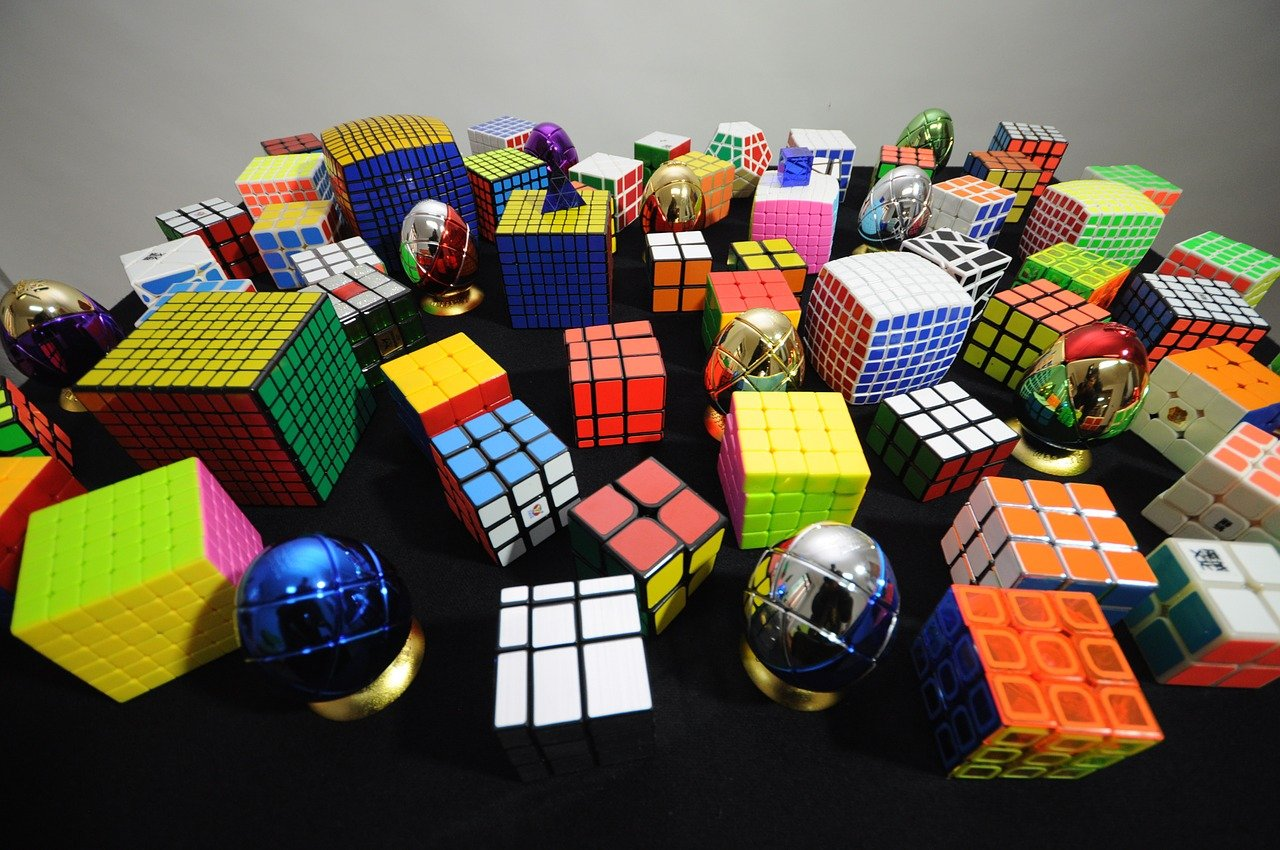
\includegraphics[scale=0.25]{pictures/rubiks.jpg}
\vspace{0,5cm}
\caption{Various Rubik's cubes}
\label{fig:cubes}
\end{figure}
\hspace{3cm}

\subsection{World records in speedcubing}
\vspace{0,5cm}

\begin{table}[h]
\centering
\begin{tabular}{|c|c|c|c|c|}
\hline
Num & Speedcuber & Record s & Date \\
\hline
1 & John Smith & 6.45 s & 01/02/2022  \\
\hline
2 & Alice Johnson & 7.12 s & 09/08/2021  \\
\hline
3 & David Brown & 7.50 s & 12/01/2020  \\
\hline
4 & Mary Davis & 7.85 s & 27/11/2019  \\
\hline
5 & Michael Wilson & 8.10 s & 22/03/2017  \\
\hline

\end{tabular}
\caption{World records in Speedcubing}
\label{tab:table1}
\end{table}
\vspace{0,5cm}
Table ~\ref{tab:table1} tells us that it is possible to solve a Rubik's cube in a few seconds!.
\vspace{0,5cm}

Typical Rubik's Cubes Brands:
\begin{itemize}
    \item MoFangGe
    \item  ShengShou
     \item YongJun
     \item Cyclone BoYs
\end{itemize}
\subsection{Pros of solving Rubik's cubes.}

Solving a Rubik's cube can teach you a lot! Here are only a few arguments for taking up this hobby:

\begin{enumerate} 
    \item \textbf{Developing logical thinking skills:} Solving a Rubik's Cube requires analysis and problem-solving. It's an excellent exercise for the mind that develops logical thinking skills.
    \item \textbf{Enhancing spatial awareness:} Manipulating the cube helps improve spatial awareness and the ability to visualize and mentally rotate objects in three-dimensional space.
    \item \textbf{Boosting patience and persistence:} Solving the Rubik's Cube can be challenging and time-consuming, teaching patience and persistence as you work towards a solution.
    \item \textbf{Stimulating creativity:} Some cubers come up with their own solving methods and algorithms, fostering creativity and problem-solving innovation.
    \item \textbf{Providing a relaxing pastime:} Solving the cube can be a meditative and relaxing activity that helps reduce stress and anxiety.
    \item \textbf{Building finger dexterity:} The fine motor skills required to manipulate the cube can improve finger dexterity and coordination.
    \item \textbf{Fostering a sense of accomplishment:} Completing a challenging puzzle like the Rubik's Cube can boost self-esteem and provide a sense of accomplishment.
    \item \textbf{Promoting healthy competition:} Competitive cubing is a global phenomenon with events and competitions, offering a chance to compete and interact with others who share the interest.
    \item \textbf{Improving memory and pattern recognition:} Memorizing solving algorithms and recognizing patterns on the cube can enhance memory and pattern recognition skills.
    \item \textbf{Providing a portable and inexpensive hobby:} The Rubik's Cube is a compact and affordable puzzle that can be enjoyed almost anywhere, making it an accessible and budget-friendly hobby.

\end{enumerate}

\vspace{0,5cm}
Thanks for reading. Hope to see you one day with a Rubik's cube in you hand!








